\section{Мета}
Отримання практичних навичок встановлення та
налаштування віртуальних машин.


\section{Завдання}
Визначити тип відеоконтролера, його режим та дату створення BIOS;
перевірити справність НМД


\section{Хід роботи}
\subsection{Код програми}
\begin{lstlisting}[language=Rust, style=colouredRust]
#include <dos.h>
#include <stdio.h>

#define VIDEO_SEG 0x0040
#define VIDEO_OFS 0x0010
#define BIOS_DATE_SEG 0xF000
#define BIOS_DATE_OFS 0xFFF5
#define NMD_SEG 0x0040
#define NMD_OFS 0x0074

void check_video_controller();
void check_bios_date();
void check_hdd_status();

void check_video_controller() {
    unsigned int config_word;
    unsigned int video_mode;

    config_word = *(unsigned int far *)MK_FP(VIDEO_SEG, VIDEO_OFS);

    video_mode = (config_word >> 4) & 3;
    switch (video_mode) {
        case 0:
            printf("Video controller type: EGA or not used.\n");
            break;
        case 1:
            printf("Video controller type: CGA, EGA, VGA in 40x25 mode.\n");
            break;
        case 2:
            printf("Video controller type: CGA, EGA, VGA in 80x25 mode.\n");
            break;
        case 3:
            printf("Video controller type: monochrome controller.\n");
            break;
        default:
            printf("Unknown video controller type.\n");
            break;
    }
}

void check_bios_date() {
    char bios_date[9];
    int i;

    for (i = 0; i < 8; i++) {
        bios_date[i] = *(char far *)MK_FP(BIOS_DATE_SEG, BIOS_DATE_OFS + i);
    }
    bios_date[8] = '\0';

    printf("BIOS creation date: %s\n", bios_date);
}

void check_hdd_status() {
    unsigned char diagnostic_byte;
    diagnostic_byte = *(unsigned char far *)MK_FP(NMD_SEG, NMD_OFS);

    if (diagnostic_byte & 8) {
            printf("NMD malfunction: unable to boot the OS from the hard disk.\n");
    } else {
        printf("NMD is in good condition.\n");
    }
}

int main() {
    check_video_controller();
    putchar('\n');
    check_bios_date();
    putchar('\n');
    check_hdd_status();
    return 0;
}    
\end{lstlisting}


\subsection{Результат роботи програми}
\begin{figure}[ht!]
    \centering
    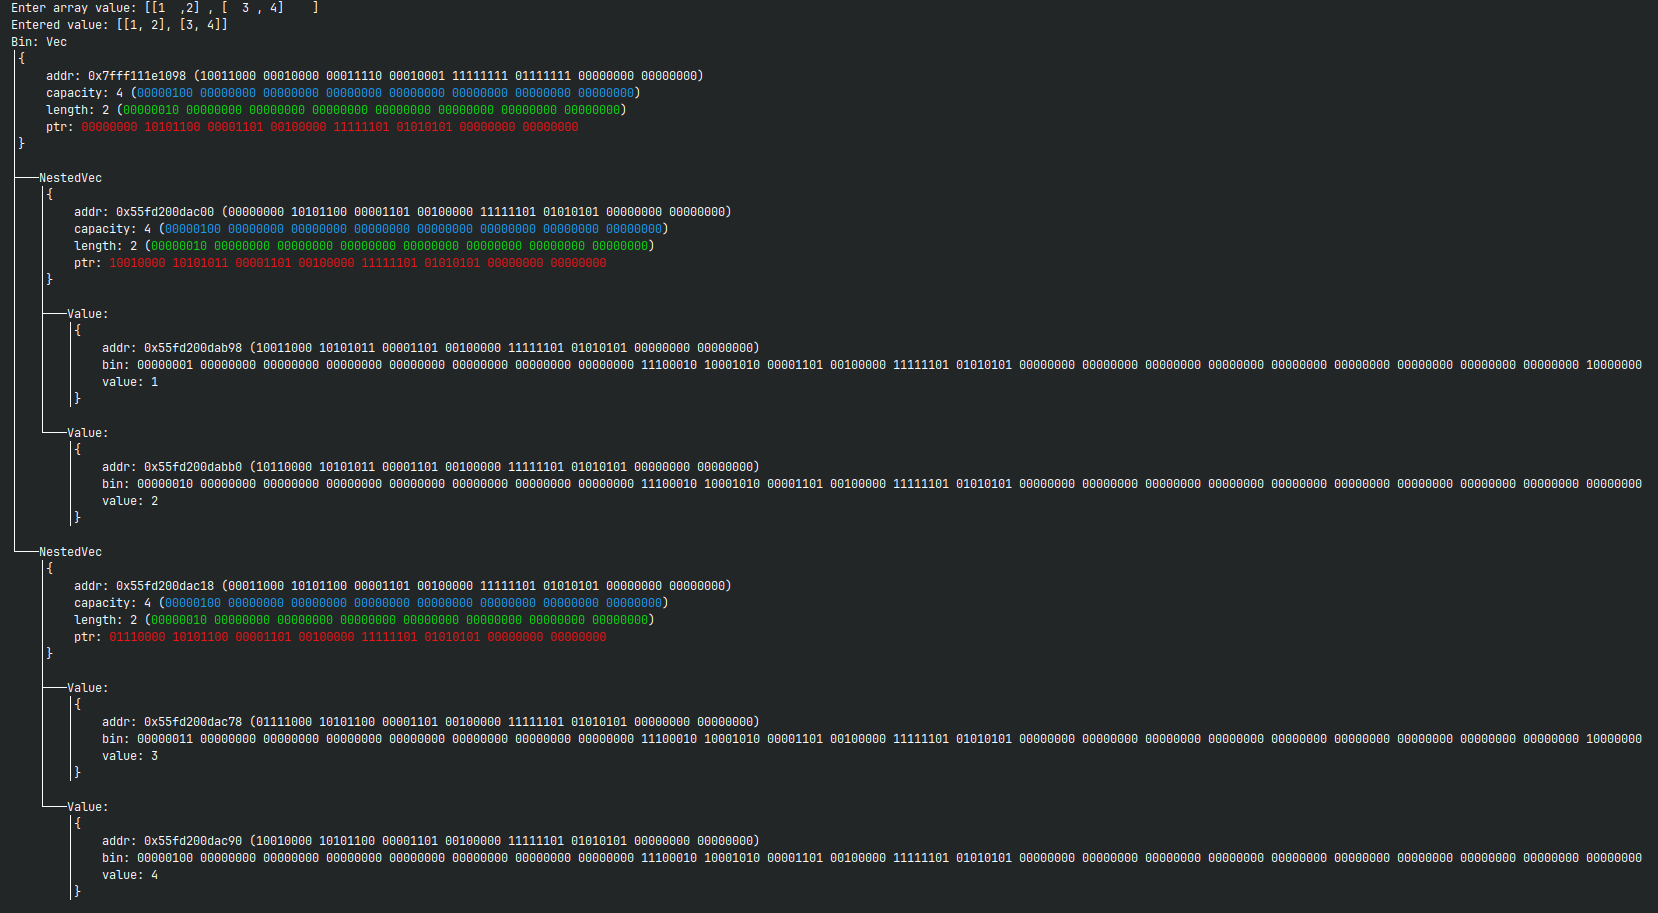
\includegraphics[width=0.9\textwidth]{\assetsDirectory/res.png}
    \caption{Результат роботи програми}
\end{figure}

\clearpage
\section{Висновки}
В ході виконання практичної роботи було отримано навички роботи з
низькорівневим доступом до системної пам'яті та аналізу конфігураційних параметрів комп'ютерної системи.
Було створено програму на мові \textbf{C}, яка зчитує слово конфігурації BIOS за адресою \texttt{0040:0010h}
і визначає тип та режим відеоконтролера, дату створення BIOS та справність НМД.
